% ============ 第八章 §2 Hensel 引理、牛顿逼近和牛顿折线 (原书 pp.275-287) ============
\section{Hensel 引理、牛顿逼近和牛顿折线}\label{sec:ch8-s2}

由上节可知, 在完备赋值域中可以使用分析工具（连续函数, 取极限等）. 本节要介绍完备非阿赋值域的重要的特殊性质.

设 $(F,P)$ 为非阿赋值域, $v$ 是 $P$ 中一个指数赋值, $O$ 和 $\mathfrak{p}$ 为其赋值环和素理想. 正则映射
\[
  O\to\overline{F}=O/\mathfrak{p},\qquad a\mapsto\bar{a}
\]
诱导出多项式环的同态
\[
  O[x]\to\overline{F}[x],\qquad f(x)=\sum a_nx^n\mapsto\bar{f}(x)=\sum\bar{a}_nx^n.
\]
如果 $\bar{f}(x)\neq 0$, 称 $f(x)$ 为 $O[x]$ 中的本原多项式. 对于 $F[x]$ 中多项式 $f(x)=a_0+a_1x+\cdots+a_nx^n$, 令
\[
  \bar{v}(f)=\min\{v(a_0),v(a_1),\cdots,v(a_n)\}.
\]
可以证明 $\bar{v}$ 是 $F(x)$ 的指数赋值并且 $\bar{v}|_F=v$, 但是我们今后不需要这个事实, 而只用 $\bar{v}$ 的上述定义. 下面结果是从 $\overline{F}$ 提升到 $O$ 的重要工具.

\begin{theorem}[\emph{Hensel 引理}]\label{thm:8.6}
设 $(F,P)$ 是完备非阿赋值域, $f(x)$ 为 $O[x]$ 中本原多项式. 如果 $\overline{f}(x)$ 在 $\overline{F}[x]$ 中分解成 $\overline{f}(x)=G(x)H(x)$, 其中 $G(x),H(x)$ 是 $\overline{F}[x]$ 中互素的多项式, 则存在 $g(x),h(x)\in O[x]$, 使得

(1) $f(x)=g(x)h(x)$;

(2) $\overline{g}(x)=G(x)$, $\overline{h}(x)=H(x)$;

(3) $\deg g(x)=\deg G(x)$.
\end{theorem}

\begin{proof}
令 $s=\deg f$, $r=\deg G(x)$, 则 $\deg\bar{f}\leqslant s$, $\deg H(x)\leqslant s-r$. 证明用逐次逼近法. 首先, 我们总可取 $g_1,h_1\in O[x]$, 使得
\[
  \bar{g}_1=G,\qquad\bar{h}_1=H,\qquad\deg g_1=\deg G,\qquad\deg h_1=\deg H.
\]
由于 $(G,H)=1$, 于是存在 $a(x),b(x)\in O[x]$, 使得 $\bar{a}G+\bar{b}H=1$, 从而 $f-g_1h_1$ 和 $ag_1+bh_1-1$ 均属于 $\mathfrak{p}[x]$. 令
\[
  \varepsilon=\min\{\bar{v}(f-g_1h_1),\bar{v}(ag_1+bh_1-1)\},
\]
则 $\varepsilon>0$. 如果 $\varepsilon=+\infty$, 则 $f=g_1h_1$ 便证明完毕. 以下设 $0<\varepsilon<\infty$. 取 $\pi\in O$, 使得 $v(\pi)=\varepsilon$. 于是
\[
  f\equiv g_1h_1\ (\mathrm{mod}\ \pi),\qquad\bar{g}_1=G,
\]
\[
  \bar{h}_1=H,\qquad\deg g_1=\deg G=r,\qquad\deg h_1\leqslant s-r.
\]
现在我们对 $i=1,2,\cdots$ 递归地构作 $g_i(x),h_i(x)\in O[x]$, 使得

(1') $f\equiv g_ih_i\ (\mathrm{mod}\ \pi^i)$;

(2') $g_i\equiv g_{i-1}\ (\mathrm{mod}\ \pi^{i-1})$, $h_i\equiv h_{i-1}\ (\mathrm{mod}\ \pi^{i-1})$（当 $i\geqslant 2$ 时）;

(3') $\deg g_i=\deg G=r$, $\deg h_i\leqslant s-r$.

前面已构作出这样的 $g_1$ 和 $h_1$. 现在设 $g_{n-1},h_{n-1}\ (n\geqslant 2)$ 满足此条件, 我们来构作 $g_n$ 和 $h_n$. 由 $(2')$ 可知应当有
\begin{equation}\tag{1}
  g_n(x)=g_{n-1}(x)+\pi^{n-1}u(x),\qquad
  h_n(x)=h_{n-1}(x)+\pi^{n-1}v(x),
\end{equation}
其中 $u(x),v(x)$ 为 $O[x]$ 中待定的多项式. 由于 $2n-2\geqslant n$, 所以
\begin{equation}\tag{2}
  \begin{aligned}
    f\equiv g_nh_n\ (\mathrm{mod}\ \pi^n)&\Leftrightarrow
    f\equiv g_{n-1}h_{n-1}+\pi^{n-1}(g_{n-1}v+h_{n-1}u)\ (\mathrm{mod}\ \pi^n)\\
    &\Leftrightarrow w\equiv g_{n-1}v+h_{n-1}u\ (\mathrm{mod}\ \pi),
  \end{aligned}
\end{equation}
其中
\[
  w=\frac{f-g_{n-1}h_{n-1}}{\pi^{n-1}}\in O[x].
\]
由于 $ag_1+bh_1\equiv 1\ (\mathrm{mod}\ \pi)$ 可知 $wag_1+wbh_1\equiv w\ (\mathrm{mod}\ \pi)$. 现在我们用下式决定 $u(x)$:
\[
  wb=q(x)g_1(x)+u(x),\qquad\deg u(x)<\deg g_1=r.
\]
由于 $G(x)$ 的最高次项系数不为 $0$, 所以 $g_1(x)$ 的最高次项系数属于 $U=O-\mathfrak{p}$. 由此可知 $u(x)\in O[x]$, 而且
\[
  (wa+qh_1)g_1+uh_1\equiv w\pmod{\pi}.
\]
将多项式 $wa+qh_1$ 中被 $\pi$ 除尽（即属于 $\pi O$）的系数均改成 $0$, 所得新的多项式叫作 $v(x)$, 则 $v(x)\in O[x]$, 并且
\begin{equation}\tag{3}
  vg_1+uh_1\equiv w\pmod{\pi}.
\end{equation}
由归纳假设知 $g_1\equiv g_{n-1}$, $h_1\equiv h_{n-1}\ (\mathrm{mod}\ \pi)$, 从而 $vg_{n-1}+uh_{n-1}\equiv w\ (\mathrm{mod}\ \pi)$. 再由 (2) 式知 $f\equiv g_nh_n\ (\mathrm{mod}\ \pi^n)$, 即 (1') 式对 $i=n$ 成立. 而由 (1) 可知 (2') 对 $i=n$ 成立. 由 $\deg u<r$ 和 (1) 式可知 $\deg g_n=\deg g_{n-1}=r$. 最后, 由 $\deg\bar{w}\leqslant s$, $\deg\bar{u}\bar{h}_1\leqslant s$, $\deg\bar{g}_1=\deg G=r$ 和 (3) 式知 $\deg\bar{v}\leqslant s-r$. 由 $v(x)$ 的构作方式知 $\deg v\leqslant s-r$. 再由 (1) 式可知 $\deg h_n\leqslant s-r$. 于是 (3') 式对 $i=n$ 也成立.

由 $(2')$ 式可知 $\lim g_n$ 和 $\lim h_n$ 存在, 并且它们的极限 $g(x)$, $h(x)$ 均属于 $O[x]$. 易知 $g(x),h(x)$ 满足定理中的 $3$ 个条件.
\end{proof}

Hensel 引理有许多应用, 比如说:

\begin{theorem}\label{thm:8.7}
设 $(F,P)$ 是完备非阿赋值域, $v$ 是 $P$ 中一个指数赋值.

(1) 若 $f(x)=a_0+a_1x+\cdots+a_nx^n$ 为 $F[x]$ 中 $n$ 次不可约多项式, 则 $\bar{v}(f)=\min\{v(a_0),v(a_n)\}$.

(2) 若 $f(x)=x^n+b_1x^{n-1}+\cdots+b_n$ 为 $F[x]$ 中不可约多项式, 则 $f(x)\in O[x]\Leftrightarrow b_n\in O$.

(3) 若 $f(x)$ 为 $O[x]$ 中首 $1$ 不可约多项式, 则 $\overline{f}(x)$ 为 $\overline{F}[x]$ 中某个不可约多项式的方幂.

(4) 设 $f(x)\in O[x]$, $\alpha\in\overline{F}$ 为 $\overline{f}(x)$ 的单根, 则存在元素 $a\in O$, 使得 $\bar{a}=\alpha$ 并且 $f(a)=0$（$\overline{f}(x)$ 在 $\overline{F}=O/\mathfrak{p}$ 中的单根均可提升成 $f(x)$ 在 $O$ 中的根）.
\end{theorem}

\begin{proof}
(1) 必要时将 $f(x)$ 乘以 $F$ 中非零元素, 可使得 $f(x)\in O[x]$ 并且 $\bar{v}(f)=0$. 我们只需证明 $v(a_0)=0$ 或者 $v(a_n)=0$. 如果 $v(a_0)$ 和 $v(a_n)$ 均为正实数, 即 $a_0,a_n\in\mathfrak{p}$, 由于 $\bar{v}(f)=0$, 可知存在 $r\ (1\leqslant r\leqslant n-1)$, 使得
\[
  v(a_r)=0,\qquad v(a_{r+1}),\cdots,v(a_n)>0.
\]
于是 $\overline{f}(x)=G(x)H(x)$, 其中 $G(x)=\overline{f}(x)$, $H(x)=1$, $\deg G=r$. 由 Hensel 引理知 $f(x)=g(x)h(x)$, 其中 $g(x),h(x)\in O[x]$, $\deg g=r$, $\deg h=n-r\geqslant 1$. 这与 $f(x)$ 在 $F[x]$ 中的不可约性相矛盾.

(2) 由 (1) 直接推出.

(3) 用反证法. 若 $\overline{f}(x)$ 在 $\overline{F}[x]$ 中有两个不同的不可约首 $1$ 多项式因子（次数均 $\geqslant 1$）, 则 $\overline{f}(x)=GH$, 其中 $G,H\in\overline{F}[x]$, $\deg G,\deg H\geqslant 1$, $(G,H)=1$. 然后由 Hensel 引理推出 $f(x)$ 在 $O[x]$ 中可约.

(4) 由条件知 $\overline{f}(x)=GH$, $G(x)=x-\alpha$. 由 $\alpha$ 为 $\overline{f}(x)$ 的单根可知 $(G,H)=1$, 再由 Hensel 引理知 $f=gh$, 其中 $g,h\in O[x]$, $g$ 为首 $1$ 多项式, 于是 $g(x)=x-a$, $a\in O$. 由 $\bar{g}=G$ 可知 $\bar{a}=\alpha$, 而 $f(a)=g(a)h(a)=0$.
\end{proof}

\begin{theorem}\label{thm:8.8}
设 $(F,P)$ 是完备非阿赋值域, 并且 $\overline{F}=O/\mathfrak{p}$ 是 $q$ 元有限域 $\F_q$, 则 $O$ 中必存在 $q-1$ 次本原单位根 $a$. 令 $T=\{0,1,a,a^2,\cdots,a^{q-2}\}$, 如果 $P$ 是离散素除子, $\pi$ 是 $F$ 的一个素元, 则 $F$ 中非零元素 $\alpha$ 均可惟一表示成
\[
  \alpha=\sum_{n=r}^{\infty}c_n\pi^n\qquad(c_n\in T,\ c_r\neq 0),
\]
其中 $r=v_P(\alpha)$.
\end{theorem}

\begin{proof}
考虑多项式 $f(x)=x^{q-1}-1\in O[x]$, 则 $\overline{f}(x)$ 在 $\overline{F}=\F_q$ 中的 $q-1$ 个根就是 $\F_q$ 的全体非零元素 $1,b,b^2,\cdots,b^{q-2}$, 其中 $b$ 是 $q-1$ 阶乘法循环群 $\F_q^{\times}$ 的生成元. 由定理 \ref{thm:8.7} 的 (4) 可知 $b$ 可以提升成 $f(x)$ 的一个根 $a\in O$, $\bar{a}=b$. 由于 $b$ 是 $q-1$ 次本原单位根, 可知 $a$ 也是 $q-1$ 次本原单位根. 并且 $\bar{a}^l=b^l\ (0\leqslant l\leqslant q-2)$ 和 $0$ 恰好是 $\overline{F}=\F_q$ 的 $q$ 个不同元素. 于是 $T$ 为 $O$ 对于 $\mathfrak{p}$ 的陪集完全代表系. 再由定理 \ref{thm:8.4} 即得 $\alpha$ 的展开式.
\end{proof}

\begin{remark}
我们知道, $p$ 进数域 $\Q_p$ 中非零元素 $\alpha$ 可以惟一表示成
\[
  \alpha=\sum_{n=r}^{\infty}c_np^n\qquad(0\leqslant c_n\leqslant p-1,\ c_r\geqslant 1),
\]
其中 $r=v_p(\alpha)$. 由于 $\Q_p$ 的剩余类域 $\Z_p/p\Z_p=\F_p$（$p$ 元域）, 由定理 \ref{thm:8.8} 知 $\Z_p$ 中存在 $p-1$ 次本原单位根 $a$. 令 $T=\{0,1,a,a^2,\cdots,a^{p-2}\}$, 则 $\alpha$ 也可以惟一表示成
\[
  \alpha=\sum_{n=r}^{\infty}a_np^n\qquad(a_n\in T,\ a_r\neq 0).
\]
\end{remark}

利用 Hensel 引理, 常常可以把 $\overline{f}(x)$ 在 $\overline{F}$ 中的根提升成 $f(x)$ 在 $O$ 中的根. 下面定理则给出求 $f(x)$ 根的一种有效的方法, 它是通常实数域 $\R=\Q_{\infty}$ 中的牛顿逐次逼近法在完备非阿赋值域中的模拟.

\begin{theorem}[\emph{牛顿逼近}]\label{thm:8.9}
设 $(F,\varphi)$ 为完备非阿赋值域, $f(x)\in O[x]$, $a_0\in O$. 如果
\[
  0<\varphi\left(f(a_0)/f'(a_0)^2\right)=r<1,
\]
令
\begin{equation}\tag{4}
  a_{i+1}=a_i-\frac{f(a_i)}{f'(a_i)}\qquad(i=0,1,2,\cdots),
\end{equation}
则

(1) 极限 $\lim a_n=\alpha\in O$ 存在, 并且 $f(\alpha)=0$.

(2) $\varphi(\alpha-a_0)\leqslant\varphi\left(\frac{f(a_0)}{f'(a_0)}\right)\leqslant\varphi\left(\frac{f(a_0)}{f'(a_0)^2}\right)=r$.
\end{theorem}

\begin{proof}
我们对 $i\geqslant 0$ 归纳证明

(A) $\varphi(a_i)\leqslant 1$（于是 $a_i\in O$）,

(B) $\varphi(a_{i+1}-a_i)=\varphi\left(\frac{f(a_i)}{f'(a_i)}\right)\leqslant\varphi\left(\frac{f(a_i)}{f'(a_i)^2}\right)\leqslant r^{2^i}$,

(C) $\varphi(a_i-a_0)\leqslant\varphi\left(\frac{f(a_0)}{f'(a_0)}\right)\leqslant r$.

在证明中还得到 $\varphi(f'(a_{i+1}))=\varphi(f'(a_i))\ (=\varphi(f'(a_0))\neq 0)$（下面 (6) 式）, 于是递归公式 (4) 可以定义.

由假设知 (A), (B) 和 (C) 对 $i=0$ 成立. 现在设它们对 $i$ 成立, 则由 (A) 和 (B) 对 $i$ 成立可知 (A) 对 $i+1$ 成立. 又由于 $a_i$ 和 $\frac{f(a_i)}{f'(a_i)}$ 均属于 $O$, 可知
\begin{align}
  \varphi(f(a_{i+1}))&=\varphi\left(f\left(a_i-\frac{f(a_i)}{f'(a_i)}\right)\right)\nonumber\\
  &=\varphi\left(f(a_i)-f'(a_i)\cdot\frac{f(a_i)}{f'(a_i)}+M\left(\frac{f(a_i)}{f'(a_i)}\right)^2\right)\nonumber\\
  &\qquad\qquad(\text{Taylor 展开}, M\in O)\nonumber\\
  &=\varphi\left(M\left(\frac{f(a_i)}{f'(a_i)}\right)^2\right)
  \leqslant\varphi\left(\frac{f(a_i)}{f'(a_i)}\right)^2.\tag{5}
\end{align}
\[
  f'(a_{i+1})=f'\left(a_i-\frac{f(a_i)}{f'(a_i)}\right)
  =f'(a_i)+M'\frac{f(a_i)}{f'(a_i)},\qquad M'\in O.
\]
于是
\[
  \frac{f'(a_{i+1})}{f'(a_i)}=1+M'\frac{f(a_i)}{f'(a_i)^2}.
\]
由于 (B) 式对 $i$ 成立, 可知
\begin{equation}\tag{6}
  \varphi\left(\frac{f'(a_{i+1})}{f'(a_i)}\right)=1.
\end{equation}
从而 $f'(a_{i+1})=f'(a_0)\neq 0$, 并且由 (5) 和 (6) 式可知
\begin{align}
  \varphi\left(\frac{f(a_{i+1})}{f'(a_{i+1})^2}\right)
  &\leqslant\varphi\left(\frac{f(a_i)}{f'(a_i)}\right)^2\varphi(f'(a_{i+1}))^{-2}\nonumber\\
  &=\varphi\left(\frac{f(a_i)}{f'(a_i)^2}\right)^2\leqslant r^{2^{i+1}},\tag{7}
\end{align}
从而 (B) 对于 $i+1$ 成立. 并且由 (7) 式可知
\[
  \varphi\left(\frac{f(a_{i+1})}{f'(a_{i+1})^2}\right)\leqslant\varphi\left(\frac{f(a_i)}{f'(a_i)^2}\right).
\]
再由 (6) 式可知
\[
  \varphi\left(\frac{f(a_{i+1})}{f'(a_{i+1})}\right)\leqslant\varphi\left(\frac{f(a_i)}{f'(a_i)}\right)\leqslant\cdots\leqslant\varphi\left(\frac{f(a_0)}{f'(a_0)}\right),
\]
即
\[
  \varphi(a_{i+1}-a_i)\leqslant\varphi(a_i-a_{i-1})\leqslant\cdots\leqslant\varphi(a_1-a_0),
\]
从而
\begin{align*}
  \varphi(a_{i+1}-a_0)&\leqslant\max\{\varphi(a_{i+1}-a_i),\varphi(a_i-a_{i-1}),\cdots,\varphi(a_1-a_0)\}\\
  &\leqslant\varphi(a_1-a_0)=\varphi\left(\frac{f(a_0)}{f'(a_0)}\right),
\end{align*}
即 (C) 式对 $i+1$ 成立. 这就证明了 (A), (B) 和 (C) 对所有 $i\geqslant 0$ 均成立.

由 (A) 和 (B) 知 $\{a_i\}$ 为 $O$ 中柯西序列. 由于 $O$ 是紧的, 从而 $\lim a_i=\alpha\in O$. 将 (B) 取极限 $i\to\infty$ 可知 $f(\alpha)=0$. 再对 (C) 式令 $i\to\infty$, 即有 $\varphi(\alpha-a_0)\leqslant\varphi\left(\frac{f(a_0)}{f'(a_0)}\right)$.
\end{proof}

采用指数赋值, 则上面定理可以改述成

\begin{theorem}\label{thm:8.10}
设 $(F,v)$ 是完备非阿赋值域, $f(x)\in O[x]$. 如果存在 $a\in O$, 使得 $2v(f'(a))<v(f(a))$, 则 $f(x)$ 在 $O$ 中有根.
\end{theorem}

作为定理 \ref{thm:8.10} 的一个应用, 我们证明

\begin{theorem}\label{thm:8.11}
(1) 设 $p$ 为奇素数, $\alpha\in\Q_p^{\times}$, $v_p(\alpha)=n$, $\alpha=p^n\cdot u$, $u=c_0+c_1p+c_2p^2+\cdots$, $0\leqslant c_i\leqslant p-1$, $c_0\neq 0$, 则
\[
  u\ \text{为 } \Q_p^{\times}\ \text{中平方元素}\Leftrightarrow n\ \text{为偶数并且 } \left(\frac{c_0}{p}\right)=1.
\]
(2) 设 $\alpha\in\Q_2^{\times}$, $v_2(\alpha)=n$, $\alpha=2^n\cdot u$, 则
\[
  \alpha\ \text{为 } \Q_2^{\times}\ \text{中平方元素}\Leftrightarrow n\ \text{为偶数并且 } u\equiv 1\ (\mathrm{mod}\ 8).
\]
\end{theorem}

\begin{proof}
(1) 若 $\alpha=\beta^2$, $\beta\in\Q_p^{\times}$, 则 $n=v_p(\alpha)=2v_p(\beta)$. 于是 $n=2m$ 为偶数. 并且 $v_p(\beta p^{-m})=0$, 于是 $\beta p^{-m}\equiv l\not\equiv 0\ (\mathrm{mod}\ p)$, 从而 $c_0\equiv u=\alpha p^{-n}=(\beta p^{-m})^2\equiv l^2\ (\mathrm{mod}\ p)$, 即 $\left(\frac{c_0}{p}\right)=1$.

反之, 若 $n=2m$ 为偶数并且 $\left(\frac{c_0}{p}\right)=1$, 则存在 $l\in\Z$, 使得 $c_0\equiv l^2\not\equiv 0\ (\mathrm{mod}\ p)$. 考虑多项式 $f(x)=x^2-u$, 则
\[
  f(l)=l^2-u\equiv l^2-c_0\equiv 0\ (\mathrm{mod}\ p),
\]
于是 $v_p(f(l))\geqslant 1$, 而 $2v_p(f'(l))=2v_p(2l)=0$. 由定理 \ref{thm:8.10} 可知 $u=a^2$, $a\in\Q_p^{\times}$, 于是 $\alpha=(ap^m)^2$, $ap^m\in\Q_p^{\times}$.

(2) 若 $\alpha=\beta^2$, $\beta\in\Q_2^{\times}$, 则 $n=v_2(\alpha)=2v_2(\beta)$. 于是 $n=2m$ 为偶数并且 $v_2(\beta 2^{-m})=0$. 于是 $\beta 2^{-m}\equiv 1\ (\mathrm{mod}\ 2)$, 从而 $u\equiv\alpha\cdot 2^{-n}=(\beta 2^{-m})^2\equiv 1\ (\mathrm{mod}\ 8)$.

反之若 $n=2m$ 为偶数并且 $u\equiv 1\ (\mathrm{mod}\ 8)$, 考虑多项式 $f(x)=x^2-u$, 则 $f(1)=1-u\equiv 0\ (\mathrm{mod}\ 8)$, 因此 $v_2(f(1))\geqslant 3$, 而 $2v_2(f'(1))=2v_2(2)=2$. 由定理 \ref{thm:8.10} 可知 $u=a^2$, $a\in\Q_2^{\times}$, 从而 $\alpha=(a2^m)^2$, $a2^m\in\Q_2^{\times}$.
\end{proof}

\begin{remark}
定理 \ref{thm:8.11} 可用来决定 $p$ 进数域 $\Q_p$ 的全部二次扩域. 和有理数域的情形一样, $\Q_p$ 是特征为 $0$ 的域. 所以 $\Q_p$ 的二次扩域均可表成 $\Q_p(\sqrt{\alpha})$, 其中 $\alpha$ 为 $\Q_p^{\times}$ 中非平方元素, 即 $\alpha\notin\Q_p^{\times^2}$. 并且 $\Q_p(\sqrt{\alpha})=\Q_p(\sqrt{\beta})$ 当且仅当 $\alpha/\beta\in\Q_p^{\times^2}$. 因此, $\Q_p$ 的二次扩域的个数等于 $\Q_p^{\times}/\Q_p^{\times^2}$ 中的元素个数减 $1$.

根据定理 \ref{thm:8.11}, 可知 $\Q_p^{\times}$ 对 $\Q_p^{\times^2}$ 的陪集代表元系可取为 $\{1,c,p,pc\}$, 其中 $c$ 是模 $p$ 的任一个非平方剩余（即 $c\in\Z$, $\left(\frac{c}{p}\right)=-1$）. 于是 $\Q_p$ 只有 $3$ 个二次扩域 $\Q_p(\sqrt{c})$, $\Q_p(\sqrt{p})$ 和 $\Q_p(\sqrt{cp})$.

若 $p=2$, 由定理 \ref{thm:8.11} 可知 $\Q_2^{\times}$ 对 $\Q_2^{\times^2}$ 的陪集完全代表系可取为 $\{1,3,5,7,2,6,10,14\}$. 所以 $\Q_2$ 共有 $7$ 个二次扩域 $\Q_2(\sqrt{c})$, 其中 $c=3,5,7,2,6,10,14$.
\end{remark}

在完备的阿基米德赋值域 $(\R,|\cdot|)$ 和 $(\C,|\cdot|)$ 中, 由多项式的系数来决定根的大小通常是困难的. 但是在完备非阿赋值域 $(F,v)$ 中, 有一种独特的方法做这件事. 设 $\Omega$ 是域 $F$ 的代数闭包, 我们在下节要证明 $v$ 在 $\Omega$ 中有惟一的扩充（定理 \ref{thm:8.15} 的注记）, 仍记为 $v$. 设
\[
  f(x)=a_0+a_1x+\cdots+a_nx^n\in F[x],\qquad a_0a_n\neq 0.
\]
平面上的点集 $S=\{(i,v(a_i))\mid 0\leqslant i\leqslant n\}$ 的下凸包络线（即它是一条折线, 其所有顶点都是 $S$ 中点, 而 $S$ 中其他点均在此折线的上方, 如图所示）叫作 $f(x)$ 的\emph{牛顿折线}. 此折线的斜率从左到右是递增的.

\begin{center}
\begin{tikzpicture}[>=stealth, scale=0.9]
  \draw[->] (-0.3,0) -- (5.3,0) node[right]{$i$};
  \draw[->] (0,-0.3) -- (0,3.6) node[above]{$v(a_i)$};
  \foreach \x/\y in {0/3, 1/1, 2/1.7, 3/0, 4/1.6}{
    \fill (\x,\y) circle (1.5pt);
  }
  \draw[thick] (0,3) -- (1,1) -- (3,0) -- (4,1.6);
\end{tikzpicture}
\end{center}

\begin{theorem}\label{thm:8.12}
设 $(r,v(a_r))$ 到 $(s,v(a_s))$ 是 $f(x)\in F[x]$ 的牛顿折线上的一条线段（$s>r$）, 斜率为 $-m$, 则

(1) $f(x)$ 在 $\Omega$ 中恰好有 $s-r$ 个根 $\alpha_1,\cdots,\alpha_{s-r}$, 使得 $v(\alpha_1)=\cdots=v(\alpha_{s-r})=m$.

(2) $f_m(x)=\prod_{i=1}^{s-r}(x-\alpha_i)\in F[x]$, 从而 $f_m(x)$ 是 $f(x)$ 在 $F[x]$ 中的一个因子.
\end{theorem}

\begin{proof}
不妨设 $a_n=1$, 即 $f(x)$ 为首 $1$ 多项式, $f(x)=\prod_{i=1}^{n}(x-\alpha_i)$, $\alpha_i\in\Omega$. 令
\[
  v(\alpha_1)=\cdots=v(\alpha_{s_1})=m_1,\qquad v(\alpha_{s_1+1})=\cdots=v(\alpha_{s_2})=m_2,\quad\cdots,
\]
\[
  v(\alpha_{s_t+1})=\cdots=v(\alpha_n)=m_{t+1},
\]
其中 $m_1<m_2<\cdots<m_{t+1}$, 则
\begin{align*}
  v(a_n)&=v(1)=0,\\
  v(a_{n-1})&\geqslant\min_{1\leqslant i\leqslant n}\{v(\alpha_i)\}=m_1\qquad(\text{因为 } -a_{n-1}=\alpha_1+\cdots+\alpha_n),\\
  v(a_{n-2})&\geqslant\min_{i\neq j}\{v(\alpha_i\alpha_j)\}=2m_1,\\
  &\cdots\\
  v(a_{n-s_1})&=\min_{i_1<\cdots<i_{s_1}}\{v(\alpha_{i_1}\cdots\alpha_{i_{s_1}})\}=v(\alpha_1\cdots\alpha_{s_1})=s_1m_1
\end{align*}
（这是由于 $\pm a_{n-s}=\sum_{i_1<\cdots<i_s}\alpha_{i_1}\cdots\alpha_{i_s}$, 而右边和式中只有一项 $\alpha_1\cdots\alpha_{s_1}$ 的指数赋值为最小值 $s_1m_1$）. 类似地,
\begin{align*}
  &v(a_{n-s_1-1})\geqslant s_1m_1+m_2,\\
  &v(a_{n-s_1-2})\geqslant s_1m_1+2m_2,\\
  &\cdots\\
  &v(a_{n-s_2})=s_1m_1+(s_2-s_1)m_2,\\
  &\cdots\\
  &v(a_0)=v(\alpha_1\cdots\alpha_n)=s_1m_1+(s_2-s_1)m_2+\cdots+(n-s_t)m_{t+1}.
\end{align*}
由这些等式和不等式不难看出, $f(x)$ 的牛顿折线的诸顶点为
\[
  (n,0),\ (n-s_1,s_1m_1),\ (n-s_2,s_1m_1+(s_2-s_1)m_2),\ \cdots,
\]
\[
  (0,s_1m_1+(s_2-s_1)m_2+\cdots+(n-s_t)m_{t+1}).
\]
顶点 $(n,0)$ 和 $(n-s_1,s_1m_1)$ 之间线段的斜率为 $\frac{0-s_1m_1}{n-(n-s_1)}=-m_1$, 对应着 $f(x)$ 有指数赋值为 $m_1$ 的 $s_1$ 个根; 顶点 $(n-s_1,s_1m_1)$ 和 $(n-s_2,s_1m_1+(s_2-s_1)m_2)$ 之间线段的斜率为 $-m_2$, 对应着 $f(x)$ 有指数赋值为 $m_2$ 的 $s_2-s_1$ 个根; $\cdots$. 由此即证明了 (1).

(2) 我们对 $\deg f=n$ 归纳. 当 $n=1$ 时命题显然成立. 现设 $\deg f=n$. 如果牛顿折线只是一条线段, 则命题也显然成立. 否则记 $s_0=0$, $s_{t+1}=n$, 则 $t\geqslant 1$. 令
\[
  f_j(x)=\prod_{i=s_j+1}^{s_{j+1}}(x-\alpha_i)\qquad(0\leqslant j\leqslant t),
\]
则 $f(x)=\prod_{j=0}^{t}f_j(x)$. 设 $g(x)$ 是 $\alpha_1$ 在 $F$ 上的最小多项式, 则 $g\mid f$. 我们在下节要证明（定理 \ref{thm:8.15}）: 若 $\Omega$ 中元素 $\alpha$ 和 $\beta$ 是 $F$-共轭的（即它们在 $F$ 上有同一个最小多项式）, 则 $v(\alpha)=v(\beta)$. 由此即知在 $\Omega[x]$ 中 $g\mid f_0$. 令 $g_1(x)=f_0/g\in\Omega[x]$, 则 $f/g=g_1\cdot\prod_{j=1}^{t}f_j\in F[x]$. 由于 $\deg f/g<n$, 由归纳假设可知 $g_1,f_j\ (1\leqslant j\leqslant t)$ 均属于 $F[x]$, 从而 $f_0=g_1g$ 也属于 $F[x]$.
\end{proof}

\begin{remark}
由定理 \ref{thm:8.12} (2) 可知, 若对某个 $i$, $s_i-s_{i-1}=1$, 即 $f(x)\in F[x]$ 只有一个根 $\alpha$ 的指数赋值为 $m_i$, 则 $\alpha$ 必然属于 $F$. 举两个例子:
\end{remark}

\begin{example}
让我们用牛顿折线法证明定理 \ref{thm:8.8}, 即设 $(F,v)$ 是完备非阿赋值域, 并且 $\overline{F}=O/\mathfrak{p}$ 为有限域 $\F_q$, 我们来证 $O$ 中必存在 $q-1$ 次本原单位根. 为此要考虑 $f(x)=x^{q-1}-1\in O[x]$. 设 $p$ 为 $q$ 的素因子（$q=p^n$）. 于是 $p=0\in\overline{F}=O/\mathfrak{p}=\F_q$, 从而 $p\in\mathfrak{p}$. 对 $q-1$ 阶乘法循环群 $\overline{F}^{\times}=\F_q^{\times}$ 的生成元 $b$, 存在 $a\in O$, 使得 $\bar{a}=b$, 于是 $a^{q-1}\equiv b^{q-1}=1\ (\mathrm{mod}\ \mathfrak{p})$, 而
\[
  f(x-a)=(x-a)^{q-1}-1\equiv\frac{(x-a)^q}{x-a}-1\equiv\frac{x^q-a^q}{x-a}-1
\]
\[
  \equiv x^{q-1}+ax^{q-2}+\cdots+a^{q-2}x+(a^{q-1}-1)\ (\mathrm{mod}\ \mathfrak{p}).
\]
但是 $a\notin\mathfrak{p}$, 从而 $v(a^i)=0\ (0\leqslant i\leqslant q-2)$, 而 $v(a^{q-1}-1)>0$. 这表明 $f(x-a)$ 的牛顿折线如左图所示, 即折线最左边线段的两端为 $(0,v(a^{q-1}-1))$ 和 $(1,0)$. 这表明 $f(x-a)$ 恰有一个根 $\alpha$, $v(\alpha)=v(a^{q-1}-1)>0$, 于是 $\alpha\in F$, 从而 $f(x)$ 在 $F$ 中有根 $\alpha+a$. 由于 $\overline{\alpha+a}=\bar{a}=b$, 可知 $\alpha+a$ 是 $F$ 中的 $q-1$ 次本原单位根.

\begin{center}
\begin{tikzpicture}[>=stealth, scale=0.9]
  \draw[->] (-0.3,0) -- (4.3,0) node[right]{$i$};
  \draw[->] (0,-0.3) -- (0,2.3) node[above]{$v$};
  \draw[thick] (0,1.6) -- (1,0) -- (3.6,0);
  \fill (0,1.6) circle (1.5pt) node[left]{$(0,v(a^{q-1}-1))$};
  \fill (1,0) circle (1.5pt) node[below]{$(1,0)$};
  \fill (2,0) circle (1.5pt);
  \fill (3,0) circle (1.5pt);
\end{tikzpicture}
\end{center}
\end{example}

\begin{example}
研究 $f(x)=a_3x^3+a_2x^2+a_1x+a_0=x^3-x^2-2x-8$ 在 $\Q_2$ 中的根（注意: $f(x)$ 是 $\Z[x]$ 中不可约多项式）.

\emph{解} $(i,v_2(a_i))\ (i=0,1,2,3)$ 分别为 $(0,3)$, $(1,1)$, $(2,0)$ 和 $(3,0)$, 于是牛顿折线有 $3$ 条边, 斜率分别为 $-2,-1,0$. 所以 $f(x)$ 的 $3$ 个根 $\alpha_1,\alpha_2,\alpha_3$ 都在 $\Q_2$ 中, 并且 $v_2(\alpha_1)=2$, $v_2(\alpha_2)=1$, $v_2(\alpha_3)=0$.

\begin{center}
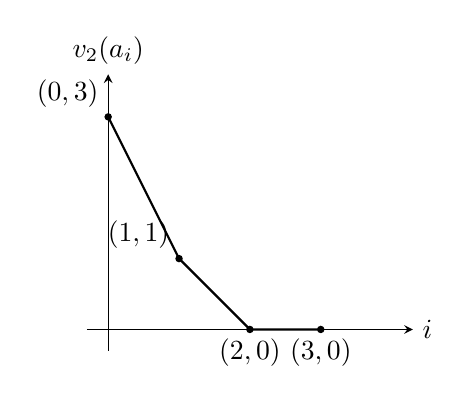
\begin{tikzpicture}[>=stealth, scale=0.9]
  \draw[->] (-0.3,0) -- (4.3,0) node[right]{$i$};
  \draw[->] (0,-0.3) -- (0,3.6) node[above]{$v_2(a_i)$};
  \draw[thick] (0,3) -- (1,1) -- (2,0) -- (3,0);
  \fill (0,3) circle (1.5pt) node[above left]{$(0,3)$};
  \fill (1,1) circle (1.5pt) node[above left]{$(1,1)$};
  \fill (2,0) circle (1.5pt) node[below]{$(2,0)$};
  \fill (3,0) circle (1.5pt) node[below]{$(3,0)$};
\end{tikzpicture}
\end{center}

我们可以用牛顿逼近法求这些根的近似值. 以下记 $v=v_2$. 根据定理 \ref{thm:8.10}, 如果存在 $a\in\Z_2$, 使得 $v(f(a))>2v(f'(a))$, 则存在 $c\in\Z_2$, 使得 $f(c)=0$, 并且 $v(c-a)\geqslant v(f(a)/f'(a))$.

取 $a=0$, 则 $v(f(0))=3>2=2v(f'(0))$. 从而由 $a=0$ 逐次逼近得到的根 $c$ 满足 $v(c-0)\geqslant v(f(0)/f'(0))=2$. 于是 $c=\alpha_1$ 迭代程序为
\[
  a_0=0,\qquad v(\alpha_1-0)\geqslant 2,
\]
\[
  a_1=a_0-\frac{f(a_0)}{f'(a_0)}=-4,\qquad v_2(\alpha_1+4)\geqslant 3,
\]
所以 $\alpha_1=2^2+\cdots$. 如果取 $a=20$, 则 $v(f(20))=7>2=2v(f'(20))$. 可知从 $a_0=20$ 出发迭代出根 $\alpha_1$, 并且 $v(\alpha_1-20)\geqslant v\left(\frac{f(20)}{f'(20)}\right)=6$. 于是 $\alpha_1=2^2+2^4+0\cdot 2^5+\cdots$. 类似地, 从 $a_0=1$ 出发迭代出 $\alpha_3$, $v(\alpha_3-87)\geqslant 7$, 于是 $\alpha_3=1+2+2^2+2^4+2^6+\cdots$; 而从 $a_0=22$ 出发得到 $v(\alpha_2-22)\geqslant 6$, 从而 $\alpha_2=2+2^2+2^4+0\cdot 2^5+\cdots$.
\end{example}

\begin{Exercises}
\item 用牛顿折线法证明定理 \ref{thm:8.11}.

\item 对每个整数 $a$, $1\leqslant a\leqslant p-1$（$p$ 为素数）, 令 $c_n=a^{p^n}$. 求证: (1) $\{c_n\}_n\ (n=0,1,2,\cdots)$ 是 $\C_p$ 中柯西序列;

(2) $\lim c_n=\alpha$ 是 $\Q_p$ 中的 $p-1$ 次单位根, 并且 $\alpha\equiv a\ (\mathrm{mod}\ p)$. 由此可知 $\Q_p$ 中存在 $p-1$ 次本原单位根.

\item 求证多项式 $f(x)=1+x^2+\frac{1}{3}x^3+3x^4$ 在 $\Q_3$ 中有根 $\alpha$, 使得 $v_3(\alpha)=-2$. 求一个有理数 $a$, 使得 $v_3(\alpha-a)\geqslant 2$.

\item 设 $(F,v)$ 是完备离散赋值域, $v$ 是标准指数赋值. $f(x)=x^n+a_{n-1}x^{n-1}+\cdots+a_0\in O[x]$, 其中 $O$ 为 $F$ 的赋值环, $n\geqslant 1$. 求证:

(1) 若 $f(x)$ 的牛顿折线是从 $(0,v(a_0))$ 到 $(n,0)$ 的一条线段, 并且 $v(a_0)$ 是和 $n$ 互素的正整数, 则 $f(x)$ 在 $F[x]$ 中不可约;

(2) （Eisenstein 判别法）若 $v(a_i)\geqslant 1\ (1\leqslant i\leqslant n-1)$, $v(a_0)=1$, 则 $f(x)$ 在 $F[x]$ 中不可约.

\item (1) 设 $p$ 为奇素数, 则 $-1$ 为 $\Q_p$ 中平方元素当且仅当 $p\equiv 1\ (\mathrm{mod}\ 4)$.

(2) 计算 $-1$ 在 $\Q_5$ 中的平方根（精确到 $5$-adic 展开的第 $4$ 位）.

\item 设 $p$ 为素数, $W_p$ 是 $\Z_p$ 中 $p-1$ 个 $p-1$ 次单位根构成的乘法循环群. $U_p=\Z_p-p\Z_p$ 是 $p$ 进单位（乘法）群. 对每个 $r\geqslant 1$, 令
\[
  U_p^{(r)}=\{u\in U_p\mid v_P(1-u)\geqslant r\}=1+p^r\Z_p
\]
（这是 $U_p$ 的乘法子群）. 求证:

(1) 当 $p\geqslant 3$ 时, $U_p=W_p\times U_p^{(1)}$（直积）;

(2) $U_2=\{\pm 1\}\times U_2^{(2)}$（直积）.
\end{Exercises}
